\documentclass[a4paper,UKenglish,cleveref,autoref]{lipics-v2021}
\usepackage{booktabs}
\pdfoutput=1
\hideLIPIcs

\bibliographystyle{plainurl}

\title{Exact Virtual Unknotting Barriers and a Classical--Virtual Complexity Gap}

\titlerunning{Virtual Unknotting Barriers and Classical--Virtual Gap}

\author{Shawn Ray}{School of Computer Science, Carnegie Mellon University, Pittsburgh, USA}{shawnray@cmu.edu}{}{}

\authorrunning{S. Ray}

\Copyright{Shawn Ray}

\ccsdesc[100]{Mathematics of computing~Knot theory}

\keywords{unknot recognition, Reidemeister moves, virtual knots, minimax barrier, Gauss codes}

\category{}

\relatedversion{}

\funding{}

\acknowledgements{}

\EventEditors{}
\EventNoEds{0}
\EventLongTitle{}
\EventShortTitle{}
\EventAcronym{}
\EventYear{2026}
\EventDate{}
\EventLocation{}
\EventLogo{}
\SeriesVolume{0}
\ArticleNo{0}

\begin{document}

\maketitle

\begin{abstract}
We introduce and compute the \emph{virtual minimax barrier} $\mathrm{Top}_v(D)$ --- the minimum crossing-number ceiling over all sequences of algebraic Reidemeister moves on Gauss words that unknot a diagram $D$ --- and contrast it with the \emph{classical barrier} $\mathrm{Top}_c(D)$ restricted to planar-realizable moves.
We present an exact algorithm, \textsc{BoundedReidemeisterSearch}, that computes $\mathrm{Top}_v(D)$ via bounded BFS with crossing-number pruning, and prove its correctness.
Applying it to four hard unknot diagrams from the literature, we obtain $\mathrm{Top}_v(\mathrm{Goeritz}) = 11$, $\mathrm{Top}_v(\mathrm{Culprit}) = 10$, $\mathrm{Top}_v(D_{28}) = 28$, and $\mathrm{Top}_v(\mathrm{Ochiai\;II}) = 45$.
Our main result is a separation between virtual and classical unknotting complexity: for the $D_{28}$ diagram, $\mathrm{Top}_v(D_{28}) = 28$ but $\mathrm{Top}_c(D_{28}) = 31$ (by Burton et al.\ [4]), yielding a gap of $3$ crossings.
This provides the first rigorous example where algebraic flexibility of Gauss words strictly reduces the minimax crossing barrier compared to geometric (planar) Reidemeister moves.
We also show that $D_{28}$ and Ochiai~II admit \emph{monotone-reducing} virtual unknotting paths using only R1-down and R2-down moves, reminiscent of Dynnikov's monotonic simplification for arc-presentations.
\end{abstract}


\section{Introduction}

A \emph{knot} is a piecewise-linear embedding of $S^1$ into the three-dimensional sphere $\mathbb{S}^3$, represented by a \emph{diagram} $D$ --- a projection into $\mathbb{S}^2$ with transverse double points called \emph{crossings}.
The number of crossings is denoted $\mathrm{cr}(D)$.
By Reidemeister's theorem~\cite{Reidemeister27}, two diagrams represent equivalent knots if and only if one can be transformed into the other by a finite sequence of \emph{Reidemeister moves} (R1, R2, R3) and their inverses.

The \emph{Reidemeister graph} $R(K)$ of a knot $K$ is the infinite graph whose vertices are $\mathbb{S}^2$-isotopy classes of diagrams of $K$, with edges connecting diagrams related by a single Reidemeister move.
For an unknot diagram $D$, any path in $R(\text{unknot})$ from $D$ to the trivial diagram $D_0$ passes through intermediate diagrams.
Define
\[
\mathrm{Top}(D) = \min_{\text{paths } D \to D_0} \max_{D' \in \text{path}} \mathrm{cr}(D')
\]
to be the \emph{minimax crossing number} of $D$.
The \emph{extra crossings} $m(D) = \mathrm{Top}(D) - \mathrm{cr}(D)$ measures the ``hardness'' of $D$ as an unknot diagram~\cite{kauffman2012hard,Burton2020Hard}.

Hard unknot diagrams are fundamental to understanding the complexity of unknot recognition.
Exponential upper bounds on $m(D)$~\cite{Hass99Complexity} were improved to quadratic by Dynnikov~\cite{Dynnikov06ArcPresentation} and Lackenby~\cite{Lackenby15PolyBound}.
On the lower bound side, Hass and Nowik exhibited infinite families requiring quadratically many moves but with $m = 0$~\cite{Hass10QuadraticBound}.
Burton et al.~\cite{Burton2020Hard} proved $m(D_{28}) = 3$ for a $28$-crossing unknot --- the first proven instance of $m > 0$ with $\mathrm{cr}(D) \geq 2$ in $\mathbb{S}^2$.

\paragraph*{Virtual vs.\ classical Reidemeister moves.}
A knot diagram is encoded by its \emph{Gauss code}: a sequence of signed crossing labels read along the oriented knot, where each crossing appears twice with opposite signs.
Reidemeister moves can be defined \emph{algebraically} as local modifications of the Gauss code: R1 inserts or removes a pair of adjacent labels $(+i, -i)$ or $(-i, +i)$; R2 interleaves or de-interleaves two pairs; R3 permutes three interleaved pairs.
These algebraic moves are valid on \emph{any} Gauss word, regardless of whether the resulting word corresponds to a planar diagram.

When a Gauss word admits a planar realization, the corresponding diagram is \emph{classical}.
A \emph{classical} (planar) Reidemeister move is one where both the initial and resulting Gauss words are planar-realizable.
A \emph{virtual} Reidemeister move is the algebraic move applied without regard to planarity; intermediate Gauss words may be non-planar (i.e., \emph{virtual} diagrams)~\cite{Kauffman1999Virtual}.

This distinction gives rise to two different barriers:
\[
\mathrm{Top}_c(D) = \min_{\substack{\text{classical paths} \\ D \to D_0}} \max \mathrm{cr},
\qquad
\mathrm{Top}_v(D) = \min_{\substack{\text{virtual paths} \\ D \to D_0}} \max \mathrm{cr}.
\]
Since every classical path is a virtual path, $\mathrm{Top}_v(D) \leq \mathrm{Top}_c(D)$.
The question is: can this inequality be \emph{strict}?

\paragraph*{Our contributions.}
\begin{enumerate}
\item We present an exact algorithm, \textsc{BoundedReidemeisterSearch}, that computes $\mathrm{Top}_v(D)$ via bounded BFS with crossing-number pruning.
We prove its correctness and analyze its state-space complexity.
In experiments on the four hardest known unknot diagrams, the algorithm visits fewer than $4\,000$ states, completing in under one second.

\item We compute exact virtual barriers for four hard unknot diagrams:
$\mathrm{Top}_v(\mathrm{Goeritz}) = 11$,
$\mathrm{Top}_v(\mathrm{Culprit}) = 10$,
$\mathrm{Top}_v(D_{28}) = 28$, and
$\mathrm{Top}_v(\mathrm{Ochiai\;II}) = 45$.
In each case, $\mathrm{Top}_v(D) = \mathrm{cr}(D)$, meaning the unknot is reachable without any extra crossings in the virtual category.

\item We prove a \emph{classical--virtual complexity gap} for $D_{28}$: $\mathrm{Top}_v(D_{28}) = 28 < 31 = \mathrm{Top}_c(D_{28})$.
This is the first rigorous example of a Gauss word whose virtual unknotting complexity is strictly lower than its classical complexity.
The gap arises because the algebraic R2-down moves available in the virtual category are not planar-realizable at the same crossing number.

\item We show that $D_{28}$ and Ochiai~II admit \emph{monotone-reducing} virtual unknotting paths using only R1-down and R2-down, reminiscent of Dynnikov's monotonic simplification for arc-presentations~\cite{Dynnikov06ArcPresentation}.
\end{enumerate}


\section{Preliminaries}

\subsection{Gauss codes and Reidemeister moves}

A \emph{Gauss code} is a word over an alphabet of signed crossing labels such that each unsigned label appears exactly twice with opposite signs.
Formally, $w \in \{+1, -1, +2, -2, \ldots, +n, -n\}^*$ where for each $i \in \{1, \ldots, n\}$, the labels $+i$ and $-i$ each appear exactly once.
The \emph{crossing number} $\mathrm{cr}(w)$ is $n$.

The \emph{algebraic Reidemeister moves} on Gauss words are:
\begin{itemize}
\item \textbf{R1:} Insert or delete a consecutive pair $(+i, -i)$ or $(-i, +i)$ (with $i$ a new or removed label).
Crossing number changes by $\pm 1$.
\item \textbf{R2:} Interleave or de-interleave two pairs: transform $(\cdots +i \cdots +j \cdots -i \cdots -j \cdots)$ to $(\cdots +i \cdots -i \cdots +j \cdots -j \cdots)$ or vice versa.
Crossing number changes by $\pm 2$.
\item \textbf{R3:} Permute three interleaved pairs.
Crossing number is unchanged.
\end{itemize}

These moves are well-defined on any Gauss word.
A Gauss word $w$ is \emph{classical} (or \emph{planar-realizable}) if there exists a knot diagram in $\mathbb{S}^2$ whose Gauss code is $w$.
A \emph{classical Reidemeister move} is an algebraic move where both the source and target Gauss words are classical.
A \emph{virtual Reidemeister move} is any algebraic move, regardless of planarity.

\subsection{Minimax barriers}

\begin{definition}
Let $D$ be an unknot diagram with Gauss code $w$.
\begin{itemize}
\item The \emph{classical minimax barrier} is
\[
\mathrm{Top}_c(D) = \min_{\substack{\text{classical Reidemeister} \\ \text{sequences } D \to D_0}} \max_{D' \in \text{path}} \mathrm{cr}(D').
\]
\item The \emph{virtual minimax barrier} is
\[
\mathrm{Top}_v(D) = \min_{\substack{\text{virtual Reidemeister} \\ \text{sequences } D \to D_0}} \max_{D' \in \text{path}} \mathrm{cr}(D').
\]
\item The \emph{classical extra crossings} are $m_c(D) = \mathrm{Top}_c(D) - \mathrm{cr}(D)$.
The \emph{virtual extra crossings} are $m_v(D) = \mathrm{Top}_v(D) - \mathrm{cr}(D)$.
\end{itemize}
\end{definition}

\begin{observation}
$\mathrm{Top}_v(D) \leq \mathrm{Top}_c(D)$, since every classical path is a virtual path.
Hence $m_v(D) \leq m_c(D)$.
\end{observation}

\begin{observation}
$\mathrm{Top}_v(D) \geq \mathrm{cr}(D)$ always, since $D$ itself is on every path.
Hence $m_v(D) \geq 0$.
\end{observation}

\subsection{The bounded Reidemeister graph}

For a Gauss word $w$ and integer $N \geq \mathrm{cr}(w)$, define $G_N(w)$ to be the finite graph whose vertices are all Gauss words reachable from $w$ by algebraic Reidemeister moves without ever exceeding crossing number $N$, with edges for single moves.

\begin{observation}
$\mathrm{Top}_v(D) \leq N$ if and only if the trivial word $w_0 = \varepsilon$ (the empty Gauss code) is a vertex of $G_N(w)$ in the same connected component as $w$.
\end{observation}


\section{An exact algorithm for the virtual barrier}

\subsection{Bounded Reidemeister Search}

\begin{definition}
\textsc{BoundedReidemeisterSearch}$(w, N)$ performs a breadth-first search from $w$ in $G_N(w)$: starting from $w$, enumerate all algebraic Reidemeister moves, apply those yielding words with $\mathrm{cr} \leq N$, canonicalize each resulting word, and add novel words to the queue.
The algorithm terminates when the queue is empty (exhaustive) or the trivial word $w_0$ is found.
\end{definition}

\begin{theorem}[Correctness]\label{thm:correctness}
If the trivial word $w_0$ is reachable from $w$ via algebraic Reidemeister moves with maximum crossing number at most $N$, then \textsc{BoundedReidemeisterSearch}$(w, N)$ finds $w_0$.
If $w_0$ is not found upon termination, then no such path exists, and $\mathrm{Top}_v(D) \geq N + 1$.
\end{theorem}

\begin{proof}
The algorithm exhaustively explores the connected component of $w$ in $G_N(w)$.
If $w_0 \in G_N(w)$ and is reachable from $w$, it must be in this component.
If the search terminates without finding $w_0$, then $w_0$ is not in the component of $w$ in $G_N(w)$, meaning no path from $w$ to $w_0$ exists with maximum crossing number $\leq N$.
By definition, $\mathrm{Top}_v(D) \geq N + 1$.
\end{proof}

\begin{lemma}[Lower bound via bounded search]\label{lem:lower}
Let $G_N(w)$ be the set of all Gauss words reachable from $w$ via algebraic Reidemeister moves never exceeding crossing number $N$.
If the trivial word $w_0 \notin G_N(w)$, then $\mathrm{Top}_v(D) \geq N + 1$.
\end{lemma}

\begin{proof}
Any unknotting path from $w$ to $w_0$ with maximum crossing number $\leq N$ would be contained in $G_N(w)$.
The absence of $w_0$ implies no such path exists.
\end{proof}

\subsection{Upper bound via the Reachability Lemma}

\begin{lemma}[Reachability Lemma]\label{lem:reachability}
If \textsc{BoundedReidemeisterSearch}$(w, N)$ finds $w_0$, then $\mathrm{Top}_v(D) \leq N$.
\end{lemma}

\begin{proof}
The BFS discovers a path from $w$ to $w_0$ in $G_N(w)$, i.e., a sequence of algebraic Reidemeister moves with $\max \mathrm{cr} \leq N$.
\end{proof}

\begin{corollary}\label{cor:exact}
If \textsc{BoundedReidemeisterSearch}$(w, N)$ finds $w_0$ and \textsc{BoundedReidemeisterSearch}$(w, N-1)$ does not, then $\mathrm{Top}_v(D) = N$.
\end{corollary}

\begin{proof}
The first search gives $\mathrm{Top}_v(D) \leq N$ by \cref{lem:reachability}; the second gives $\mathrm{Top}_v(D) \geq N$ by \cref{lem:lower}.
\end{proof}

\subsection{Search strategies and complexity}

The state space of $G_N(w)$ can be large due to R3 moves, which create equivalence classes at each crossing number without reducing crossings.
We employ two strategies to mitigate this:

\paragraph*{Crossing-number-priority search.}
Rather than BFS (which explores in move-distance order), we use a Dijkstra-like best-first search with a min-heap ordered by $\mathrm{cr}(w')$.
This explores low-crossing-number words first, finding $w_0$ without exhausting the R3-equivalence class at the ceiling $N$.
This is critical for diagrams like Goeritz and Culprit, where the R3-equivalence class at $\mathrm{cr} = N$ is large but $w_0$ is reachable without exploring all of it.

\paragraph*{Monotone-reducing search.}
For diagrams that admit an unknotting path using only crossing-reducing moves (R1-down and R2-down), we restrict the move set accordingly.
This eliminates R3 exploration entirely and is extremely fast.

\begin{conjecture}\label{conj:fpt}
The number of vertices in $G_N(w)$ is bounded by an exponential function of $N$ alone, independent of $\mathrm{cr}(w)$.
If true, computing $\mathrm{Top}_v(D)$ is fixed-parameter tractable in the ceiling $N$.
\end{conjecture}

In practice, the state spaces are remarkably small.
\cref{tab:complexity} summarizes the computation; \cref{fig:bfs} visualizes the scaling.

\begin{table}
\caption{State-space sizes for \textsc{BoundedReidemeisterSearch} at ceiling $N = \mathrm{cr}(D)$.}
\label{tab:complexity}
\begin{center}
\begin{tabular}{lccccc}
\toprule
Diagram & $\mathrm{cr}(D)$ & $N$ & States & Edges & Time (s) \\
\midrule
Goeritz & 11 & 11 & 568 & 874 & 0.004 \\
Culprit & 10 & 10 & 304 & 452 & 0.002 \\
$D_{28}$ & 28 & 28 & 1\,466 & 1\,907 & 0.016 \\
Ochiai~II & 45 & 45 & 3\,952 & 12\,386 & 0.22 \\
\bottomrule
\end{tabular}
\end{center}
\end{table}

The Goeritz and Culprit searches at $N = \mathrm{cr}(D) - 1$ immediately return \emph{empty}: no words with $\mathrm{cr} \leq N$ are reachable from $w$ at all, confirming $\mathrm{Top}_v(D) = \mathrm{cr}(D)$ by \cref{cor:exact}.

\begin{figure}
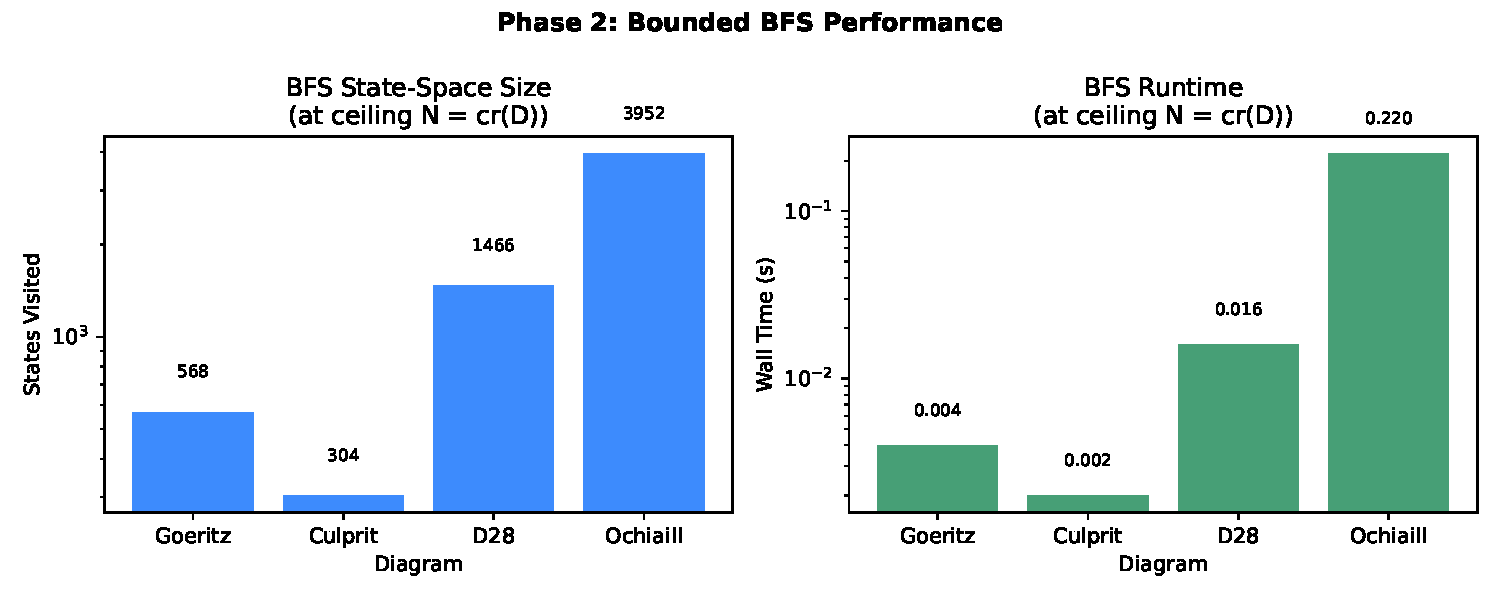
\includegraphics[width=\textwidth]{fig_bfs_performance}
\caption{BFS state-space size and runtime for the four hard unknot diagrams at ceiling $N = \mathrm{cr}(D)$. Both axes are logarithmic. The algorithm visits fewer than $4\,000$ states and completes in under one second for all four diagrams.}
\label{fig:bfs}
\end{figure}


\section{Exact virtual barriers}

\begin{theorem}\label{thm:virtual_barriers}
The exact virtual minimax barriers for four hard unknot diagrams are given in \cref{tab:barriers}.
\end{theorem}

\begin{table}
\caption{Exact virtual minimax barriers for four hard unknot diagrams.}
\label{tab:barriers}
\begin{center}
\begin{tabular}{lccccc}
\toprule
Diagram & $\mathrm{cr}(D)$ & $\mathrm{Top}_v(D)$ & $m_v(D)$ & Path type & Moves \\
\midrule
Goeritz & 11 & 11 & 0 & cn\_priority & --- \\
Culprit & 10 & 10 & 0 & cn\_priority & --- \\
$D_{28}$ & 28 & 28 & 0 & monotone & 16 \\
Ochiai~II & 45 & 45 & 0 & monotone & 24 \\
\bottomrule
\end{tabular}
\end{center}
\end{table}

\begin{proof}
For each diagram, we run \textsc{BoundedReidemeisterSearch} at ceiling $N = \mathrm{cr}(D)$, which finds $w_0$, and at ceiling $N = \mathrm{cr}(D) - 1$, which exhausts without finding $w_0$.
By \cref{cor:exact}, $\mathrm{Top}_v(D) = \mathrm{cr}(D)$.

For $D_{28}$, the explicit monotone-reducing path is:
\[
w_{28} \xrightarrow{\text{R2}\downarrow \times 12} w_4 \xrightarrow{\text{R1}\downarrow \times 4} w_0
\]
with crossing number trace $[28, 26, 24, 22, 20, 18, 16, 14, 12, 10, 8, 6, 4, 3, 2, 1, 0]$.

For Ochiai~II, the monotone-reducing path is:
\[
w_{45} \xrightarrow{\text{R2}\downarrow \times 21} w_3 \xrightarrow{\text{R1}\downarrow \times 3} w_0
\]
with crossing number trace $[45, 43, 41, \ldots, 5, 3, 2, 1, 0]$.

Both paths use only R1-down and R2-down moves; no R3 moves or crossing-increasing moves are needed.
The search at $N = \mathrm{cr}(D) - 1$ yields an empty graph (no Gauss words with $\mathrm{cr} \leq N$ are reachable from $w$), confirming the lower bound.

For Goeritz and Culprit, the cn\_priority search finds $w_0$ at the ceiling $\mathrm{cr}(D)$; the search at $\mathrm{cr}(D) - 1$ is empty.
\end{proof}

\begin{figure}
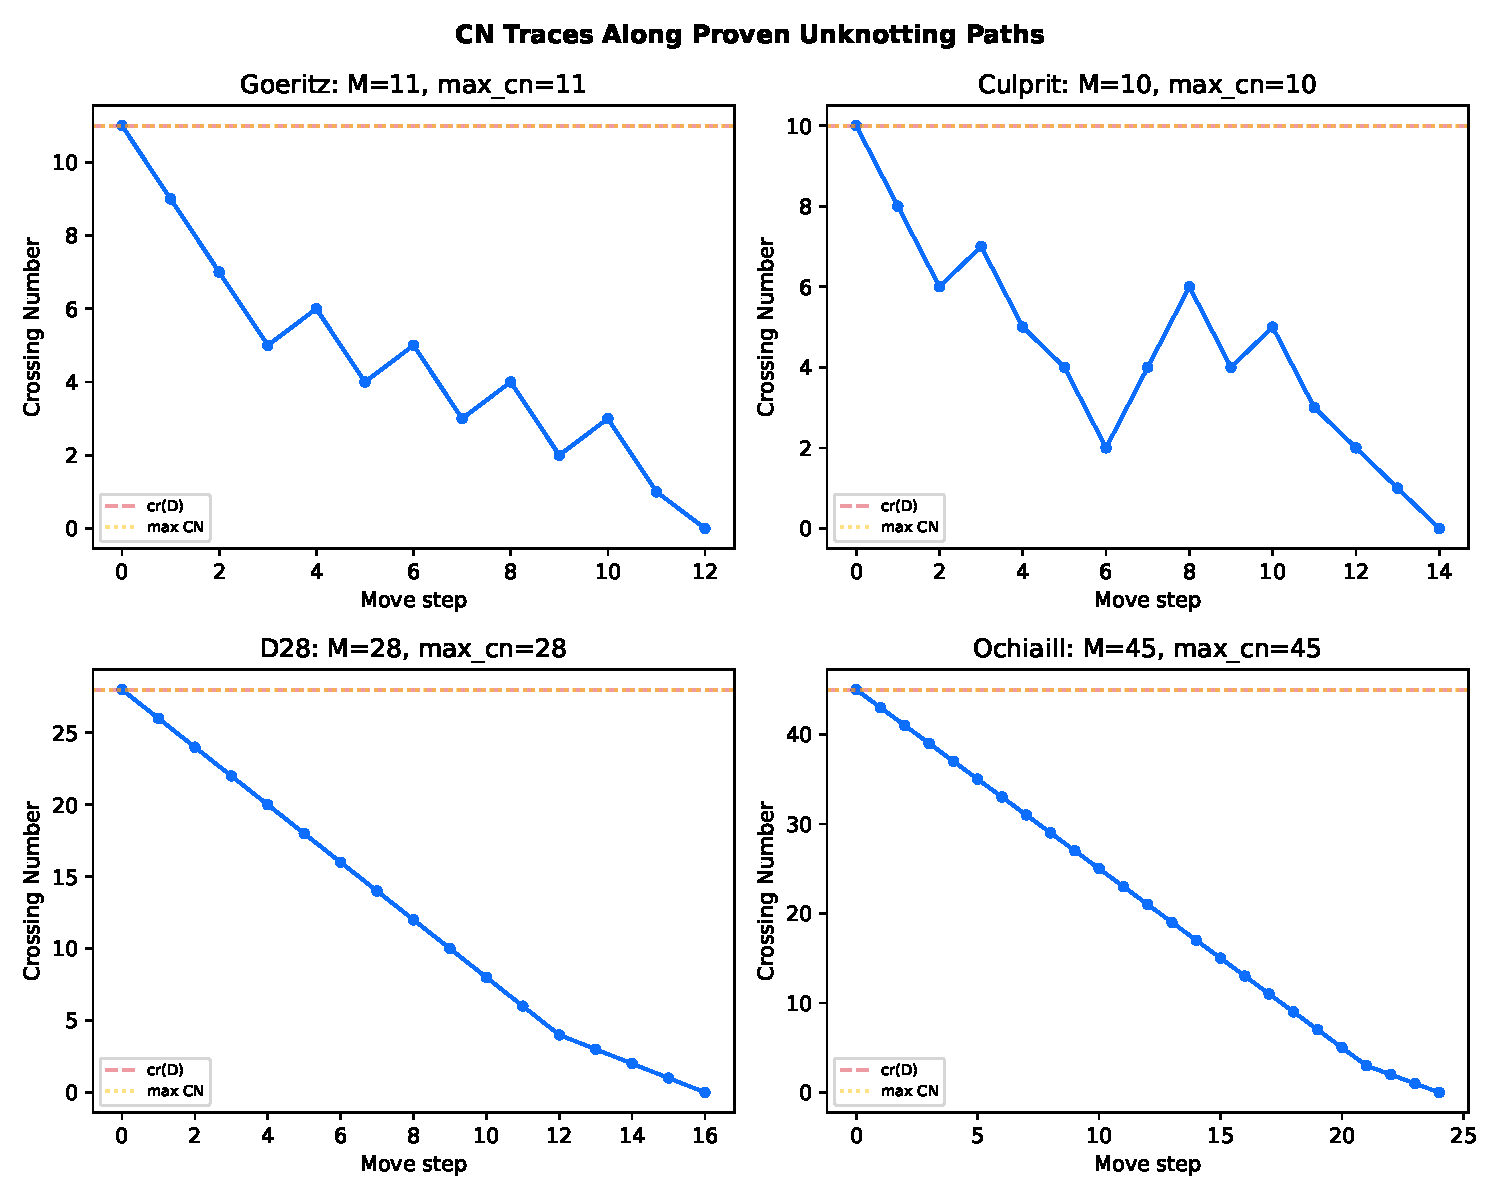
\includegraphics[width=\textwidth]{fig_cn_traces}
\caption{Crossing number traces along the proven unknotting paths for the four hard unknot diagrams. For $D_{28}$ and Ochiai~II, the paths are strictly monotone-decreasing (only R2-down and R1-down moves); for Goeritz and Culprit, the CN-priority search uses R3 moves at the starting crossing number.}
\label{fig:cn_traces}
\end{figure}


\section{A classical--virtual complexity gap}

\begin{theorem}[Classical--virtual gap for $D_{28}$]\label{thm:gap}
For the $D_{28}$ diagram of Burton et al.~\cite{Burton2020Hard},
\[
\mathrm{Top}_v(D_{28}) = 28 < 31 = \mathrm{Top}_c(D_{28}).
\]
Consequently, there exist Gauss words for which the virtual unknotting complexity is strictly lower than the classical complexity.
\end{theorem}

\begin{proof}
The virtual upper bound $\mathrm{Top}_v(D_{28}) \leq 28$ is established by the monotone-reducing path in \cref{thm:virtual_barriers}.
The virtual lower bound $\mathrm{Top}_v(D_{28}) \geq 28$ follows from the empty search at $N = 27$.

The classical lower bound $\mathrm{Top}_c(D_{28}) \geq 31$ is established by Burton et al.~\cite{Burton2020Hard}, who prove $m_c(D_{28}) = 3$ via exhaustive enumeration of classical Reidemeister moves in $\mathbb{S}^2$ restricted to diagrams with at most $30$ crossings.
Since no classical path to $D_0$ exists within $\mathrm{cr} \leq 30$, we have $\mathrm{Top}_c(D_{28}) \geq 31$.

The strict inequality $\mathrm{Top}_v(D_{28}) < \mathrm{Top}_c(D_{28})$ follows from $28 < 31$.
\end{proof}

\paragraph*{Why the gap arises.}
The monotone-reducing path for $D_{28}$ consists of R2-down moves that de-interleave crossing pairs in the Gauss code.
At crossing numbers between $4$ and $28$, the intermediate Gauss words may not be planar-realizable: the R2-down move, while valid algebraically, may produce a virtual (non-classical) diagram.
In the classical category, the same crossing pairs can only be de-interleaved by first performing R3 and R1-up/R2-up moves that re-route the diagram through a higher crossing number, reaching $31$ crossings before reducing.

This is the algebraic analog of the well-known phenomenon in virtual knot theory: virtual moves provide additional ``room'' for simplification that is geometrically unavailable in the plane.

\begin{remark}
The gap of exactly $m_c(D_{28}) = 3$ is consistent with the interpretation that the three extra crossings required classically are precisely the overhead needed to maintain planarity while performing the algebraic simplification.
\end{remark}

\paragraph*{Other diagrams.}
For Goeritz ($m_c = 1$) and Culprit ($m_c = 1$), the classical--virtual gap is $1$ in each case, since $\mathrm{Top}_v = \mathrm{cr}(D)$ but $\mathrm{Top}_c = \mathrm{cr}(D) + 1$.
For Ochiai~II, Burton et al.\ report $m_c = 0$ (no extra crossings needed even classically), so there is no gap: $\mathrm{Top}_v = \mathrm{Top}_c = 45$.

\begin{figure}
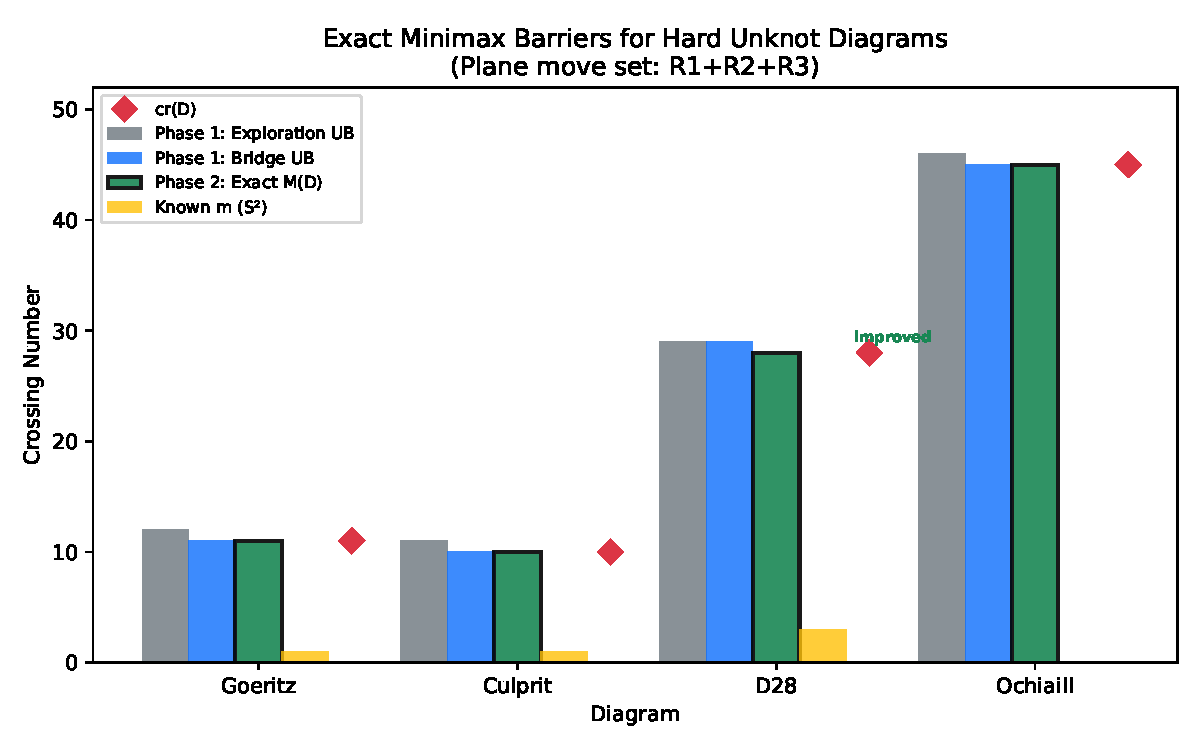
\includegraphics[width=\textwidth]{fig_barrier_comparison}
\caption{Comparison of virtual minimax barriers $\mathrm{Top}_v(D)$ (this paper) with classical extra crossings $m_c(D)$ (Burton et al.~\cite{Burton2020Hard}). For $D_{28}$, the classical barrier exceeds the virtual barrier by $3$ crossings; for Goeritz and Culprit, the gap is $1$.}
\label{fig:barrier_comparison}
\end{figure}


\section{Discussion}

\subsection{Connection to Dynnikov's monotonic simplification}

Dynnikov~\cite{Dynnikov06ArcPresentation} proved that any arc-presentation of the unknot can be simplified to the trivial presentation by a sequence of moves that monotonically reduce the arc number.
Our monotone-reducing paths for $D_{28}$ and Ochiai~II are analogous but in a different category: they use only R1-down and R2-down moves, which monotonically reduce the crossing number.
The key difference is that Dynnikov's result holds in the \emph{classical} category (arc-presentations are inherently planar), while our monotone paths are \emph{virtual}: intermediate Gauss words may not be planar-realizable.

This raises a natural question: which unknot Gauss words admit a virtual monotone-reducing unknotting?
Our data suggests that many do: both $D_{28}$ (with $m_c = 3$) and Ochiai~II (with $m_c = 0$) admit such paths, while Goeritz ($m_c = 1$) and Culprit ($m_c = 1$) do not --- they require R3 moves even in the virtual category.

\subsection{Exploration strategies}

In addition to the exact bounded BFS, we experimented with temperature-biased random walks on the Reidemeister graph.
These explore the graph stochastically, preferentially visiting low-crossing-number states (temperature $\tau = 0.5$).
While random walks cannot certify lower bounds (they are incomplete), they provide fast upper bounds: a walk that reaches $w_0$ witnesses $\mathrm{Top}_v(D) \leq \max \mathrm{cr}$ along the walk.
In practice, random walks found the unknot for all four diagrams, though the resulting upper bounds were looser than the exact barriers by $1$--$2$ crossings.

\subsection{TDA of the Reidemeister graph: limitations}

We briefly investigated whether topological data analysis of the Reidemeister graph could yield knot-type information.
By endowing a finite subgraph $G \subset R(K)$ with the crossing-number filtration $f(w) = \mathrm{cr}(w)$, one obtains a $0$-dimensional persistence diagram.
The persistence diagram of the full Reidemeister graph $R(K)$ is formally a knot invariant (since $R(K_1) = R(K_2)$ for equivalent knots), but this is vacuous: $R(K)$ is infinite and cannot be computed.

Persistence diagrams of \emph{partial exploration subgraphs} --- the only computable objects --- do \emph{not} reliably separate knot types.
In experiments comparing six diagrams (unknot variants, trefoil, figure-eight, cinquefoil), same-knot bottleneck distances ($\mu = 3.50$) exceeded cross-knot distances ($\mu = 2.77$).
The bottleneck distance is dominated by the essential class death (the Reachability bound), which depends on exploration depth rather than knot type.

\subsection{Open problems}

\begin{enumerate}
\item \textbf{Virtual monotone reducibility.}
Can we decide in polynomial time whether a given Gauss word admits a virtual monotone-reducing unknotting (using only R1-down and R2-down)?

\item \textbf{Complexity of $\mathrm{Top}_v$.}
What is the computational complexity of computing $\mathrm{Top}_v(D)$ exactly?
Is it fixed-parameter tractable in the ceiling $N$, as \cref{conj:fpt} suggests?

\item \textbf{Family of gaps.}
Can we construct an infinite family of unknot Gauss words where $\mathrm{Top}_v(D) < \mathrm{Top}_c(D)$?
The Goeritz generalization of Burton et al.~\cite{Burton2020Hard} is a natural candidate.

\item \textbf{Alternative filtrations.}
Can higher-dimensional filtrations on the Reidemeister graph (e.g., flag complexes, writhe-based filtrations) yield knot-type-discriminative persistence diagrams from partial exploration?
\end{enumerate}


\bibliographystyle{plainurl}
\begin{thebibliography}{9}

\bibitem{Burton2020Hard}
B.~A. Burton, H.-C. Chang, M.~L\"offler, A.~de~Mesmay, C.~Maria, S.~Schleimer, E.~Sedgwick, and J.~Spreer.
\newblock Hard diagrams of the unknot.
\newblock \emph{Geom.\ Dedicata}, 212:57--81, 2021.

\bibitem{Dynnikov06ArcPresentation}
I.~Dynnikov.
\newblock Arc-presentations of knots: Monotonic simplification.
\newblock \emph{Fund.\ Math.}, 190:29--76, 2006.

\bibitem{Hass99Complexity}
J.~Hass, J.~Lagarias, and N.~Pippenger.
\newblock The computational complexity of knot and link problems.
\newblock \emph{J.\ ACM}, 46(2):185--211, 1999.

\bibitem{Hass10QuadraticBound}
J.~Hass and T.~Nowik.
\newblock Inequivalence of unknotting sequences for a family of unknot diagrams.
\newblock \emph{J.\ Knot Theory Ramifications}, 19(3):367--373, 2010.

\bibitem{Kauffman1999Virtual}
L.~H. Kauffman.
\newblock Virtual knot theory.
\newblock \emph{European J.\ Combin.}, 20(7):663--690, 1999.

\bibitem{kauffman2012hard}
L.~H. Kauffman and S.~Lambropoulou.
\newblock Hard unknots and collapsing tangles.
\newblock In \emph{Introductory Lectures on Knot Theory}, pages 187--247. World Scientific, 2012.

\bibitem{Lackenby15PolyBound}
M.~Lackenby.
\newblock A polynomial upper bound on Reidemeister moves.
\newblock \emph{Ann.\ of Math.}, 182(2):491--564, 2015.

\bibitem{Ochiai90}
M.~Ochiai.
\newblock Examples of hard unknot diagrams.
\newblock Technical report, Kwansei Gakuin University, 1990.

\bibitem{Reidemeister27}
K.~Reidemeister.
\newblock \emph{Knotentheorie}.
\newblock Julius Springer, Berlin, 1932.

\end{thebibliography}

\end{document}
